\chapter{Definição do Modelo}
\label{chap:modelo}

\todo{"Você precisa definir primeiramente um polígono através de images"}

\todo{"Através de uma sequência de imagens, mostre como você usa o conceito de polígonos para crir as IDRs e depois sobrepor durante o tempo para identificar as diferências"}

Neste capítulo, entendemos o que são as Regiões Densas Interessantes e definimos o modelo espaço-temporal.

\section{Regiões Densas Interessantes}

\abrv[IDR \qquad Interesting Dense Region]{}

Uma Região Densa Interessante (do inglês {\em Interesting Dense Region}, IDR) é uma região espacial com uma alta probabilidade de conter pontos de interesse do analista. IDR são coletadas e definidas durante o processamento do feedback do usuário. Diferentemente da literatura que predominantemente foca em interações explícitas, como clicar no botão, abrir o perfil do ponto, investigamos o feedback implícito.

Durante a exploração iterativa de dados espaciais, é comum o caso que o analista avalia algumas regiões de interesse, mas esquece de dá um feedback explícito sobre aquela região. O ato do usuário olhar para essa região pode ser capturado através do rastreio da movimentos oculares e, como \citeonline{arapakis2014user} comprova, esse método possui uma forte relação com a atenção do usuário.

Entretanto o rastreamento dos movimentos oculares fere várias questões de privacidade, assim sendo optamos pela alternativa de rastrear os deslocamentos do cursor do mouse. \citeonline{arapakis2014understanding} argumenta que esse método possui uma forte relação com o engajamento do usuário. Intuitivamente, um ponto espacial recebe um feedback positivo se o cursor do mouse se desloca próximo a ele frequentemente.

O objetivo de descobrir IDRs é para obter preferências do analista que nunca foram expressadas explicitamente. Para tal, baseamos em dois conceitos:

\begin{itemize}
	\item \textbf{Conceito 1}: uma região é mais interessante ao analista, se for densa. Por exemplo, o analista movimenta seu mouse naquela regiãos várias vezes.
	\item \textbf{Conceito 2}: é possível que o analista movimente seu mouse em qualquer lugar do mapa. Isso não deve significar que todo lugar no mapa tem a mesma significância.
\end{itemize}


\subsection{Perfil}

Uma IDR descreve uma região espacial do conjunto de dados do analista coletada num determinado tempo $t$. Essa região representa as preferências do analista no momento $t$ no contexto espacial, ou seja, onde o analista está interessado. Para entender, em quê o analista está interessado, definimos o perfil dessa região.

\begin{table}[]
	\centering
	\begin{tabular}{|l|l|}
		\hline
		\textbf{id}                  & 15                             \\ \hline
		\textbf{latitude}            & 48.88880                       \\ \hline
		\textbf{longitude}           & 2.320465                       \\ \hline
		\textbf{name}                & Nice appartment in Batignolles \\ \hline
		\textbf{host\_name}          & Daniele                        \\ \hline
		\textbf{neighbourhood}       & Batignolles-Monceau            \\ \hline
		\textbf{room\_type}          & Entire home/apt                \\ \hline
		\textbf{price}               & 65                             \\ \hline
		\textbf{minimun\_nights}     & 1                              \\ \hline
		\textbf{stars}               & 4                              \\ \hline
		\textbf{number\_of\_reviews} & 25                             \\ \hline
		\textbf{reviews\_per\_month} & 1.74                           \\ \hline
		\textbf{availability\_365}   & 35                             \\ \hline
		\textbf{last\_review}        & 2015-11-14T09:07:01+00:00      \\ \hline
	\end{tabular}
	\caption{Exemplo de atributos de um ponto que representa uma estadia}
	\label{table:atributos}
\end{table}

O perfil é a sumarização dos atributos dos pontos contidos numa IDR. Cada ponto em um conjunto de dados ($p \in \mathcal{P}$) é descrito por suas coordenadas espaciais e uma série de atributos de domínio $dom(p)$. A Tabela \ref{table:atributos} apresenta um exemplo dos atributos de um ponto no conjunto de dados do Airbnb.

Na Tabela \ref{table:atributos}, os atributos {\em latitude} e {\em longitude} são as coordenadas espaciais, enquanto que todos os outros atributos caracterizam os atributos de domínio. Dentre os atributos de domínio, podemos encontrar 4 tipos:

\begin{enumerate}
	\item Numéricos: são atributos que representam valores numéricos, como, por exemplo, os atributos {\em price}, {\em minimun\_nights}, {\em number\_of\_reviews}, {\em reviews\_per\_month} e {\em availability\_365}.
	\item Textuais: são atributos que representam valores textuais, como, por exemplo, os atributos {\em name} e {\em host\_name}.
	\item Categóricos: são atributos que representam valores tanto numéricos, quanto textuais, mas que se repetem pouco em todo o conjunto. Por exemplo, o atributo {\em stars} possue apenas cinco valores em todo o conjunto. Os atributos {\em room\_type} e {\em neighbourhood} também possuem um número finito de opções, por isso são classificados como categorias.
	\item Temporais: são atributos que representam data e/ou hora, como, por exemplo, o atributo {\em last\_review} que representa quando foi publicado a última avaliação.
\end{enumerate}

Esses 4 tipos são comumente encontrados em conjuntos de dados espacias, portanto o perfil da IDR precisa representar de maneira resumida esses atributos em relação aos pontos nela contidos. Assim sendo, tratamos cada tipo de acordo com sua especificidade:

% Os atributos {\em name} e {\em host_name} são atributos textuais. Os atributos 

\begin{figure}[t]
	\centering
	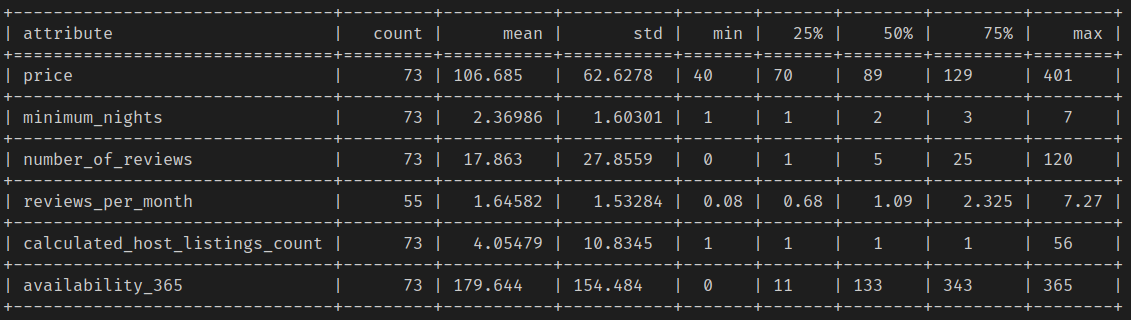
\includegraphics[width=\columnwidth]{imagens/perfil-numericos}
	\caption{Perfil dos atributos numéricos de uma IDR}
	\label{fig:perfil-numericos}
	\vspace{-10pt}
\end{figure}

\begin{figure}[t]
	\centering
	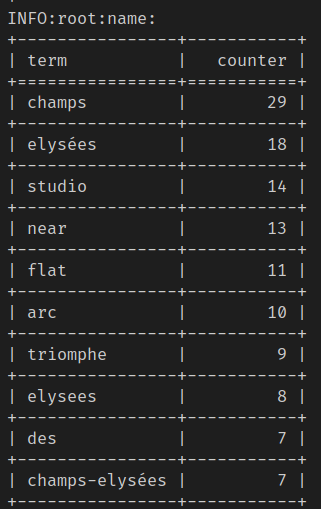
\includegraphics[height=10cm,keepaspectratio]{imagens/perfil-textuais}
	\caption{Perfil do atributo textual de uma IDR}
	\label{fig:perfil-textuais}
	\vspace{-10pt}
\end{figure}

\begin{figure}[t]
	\centering
	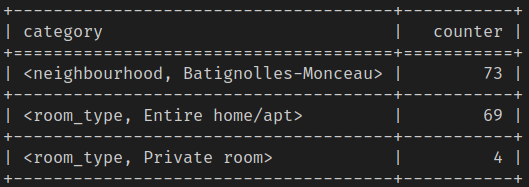
\includegraphics[width=\columnwidth]{imagens/perfil-categoricos}
	\caption{Perfil dos atributos categóricos de uma IDR}
	\label{fig:perfil-categoricos}
	\vspace{-10pt}
\end{figure}

\begin{enumerate}
	\item Numéricos: os atributos números encontrados me uma IDR são sumarizados usando funções estatísticas como média, desvio padrão, mínimo e máximo. Podemos ver um exemplo do resultado dessa sumarização na Figura \ref{fig:perfil-numericos}.

	\item Textuais: os atributos textos são tratados separadamente. Para cada atributo, é feito o levantamento dos termos mais usados. Essa abordagem é utilizado por \citeonline{kumar2017} para encontrar os termos mais usados no contexto temporal. A Figura \ref{fig:perfil-textuais} apresenta o resultado para o atributo {\em name} em uma IDR.

	\item Categóricos: os atributos categóricos são contabilizados num dicionário $M$ onde as chaves são uma tupla com o nome do atributo e o valor da categoria. Quanto maior a quantidade de repetições de uma categoria, mais relevante no contexto de uma IDR. A Figura \ref{fig:perfil-categoricos} mostra o resultado num conjunto de dados para os atributos {\em neighbourhood} e {\em room\_type}.

	\item Temporais: os atributos temporais são normalizados para uma escala linear (a partir do ano novo para datas e a partir da meia noite para horas) a fim de ser contabilizado as ocorrências. Por exemplo, uma atributo com a data {\em 2018-12-21} é normalizado para {\em 2018, 12, 355}, isto é, numa linha temporal esse evento ocorreu no ano 2018, no 12º mês e no 355º dia. As horas são normalizados de maneira similiar, a hora {\em 08:33:22} é normalizado para {\em 8, 513, 30802}, isto é, esse evento ocorreu no 8º hora, 513º minuto e 30802º segundo. Com os valores normalizadas, criamos um histograma e encontrar os dias e os momentos do dia mais presente na IDR.
\end{enumerate}


\section{Modelo Temporal}

Cada IDR é coletado num momento $t$ e seu perfil definido através dos atributos de domínio dos pontos contidos na região delimitada. Dessa forma, para cada momento $t$ em qualquer espaço de tempo, sabemos as preferências do usuário tanto no contexto espacial quanto no contexto de domínio.

O perfil pode ser definido para cada IDR, mas também para um conjunto de IDRs, ou seja, é possível realizar a análise das preferências do analista em qualquer espaço de tempo (minutos, horas, dias, semanas etc).

Assim sendo é através das IDRs coletadas que podemos aplicar a análise temporal e evoluir o sistema de destacamente de informação do GeoGuide.